\documentclass{article}

\usepackage{graphicx}
\usepackage{amsmath}
\usepackage{caption}
\usepackage{subcaption}
\usepackage{listings}
\usepackage[hidelinks]{hyperref}
\usepackage{enumitem}
\usepackage{geometry}
\usepackage{biblatex}

\renewcommand{\contentsname}{Table of Contents}
\addbibresource{sad.bib}
\geometry{
 a4paper,
 left=20mm,
 right=20mm,
 top=20mm,
 bottom=25mm,
 }

\begin{document}

\begin{titlepage}
\begin{center}
\vspace*{1cm}

\Huge
\textbf{Project 01: Home Safe}

\vspace{0.5cm}
\Large
\textit{Software Architecture Design} \\
\textit{SAD Version 3}

\vspace{1cm}

\textbf{Team 01}

\vspace{0.5cm}

\text{Marina Seheon (Manager)} \\
\text{Andrei Phelps (Document Manager)} \\
\text{Luke McDougall (Lead Software Engineer)} \\
\text{Jack Vanlyssel} \\
\text{Spoorthi Menta} \\
\text{Vamsi Krishna Singara} \\

\vspace{1cm}

\begin{figure}[h]
    \centering
    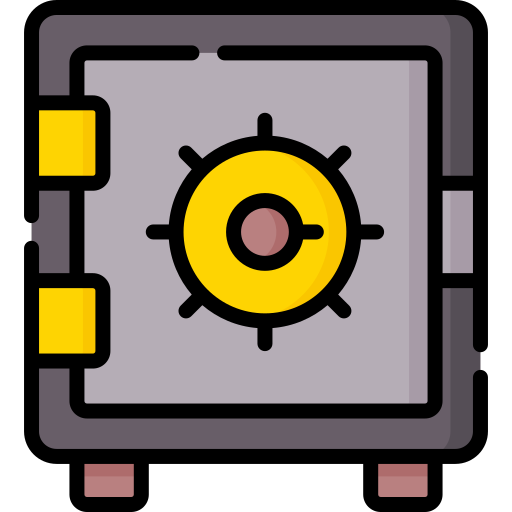
\includegraphics[width=0.25\textwidth]{docs/figs/safe.png}
    \caption*{Image courtesy of Flaticon.com \cite{flaticonSafeDeposit}.}
    \label{fig:safeIcon}
\end{figure}

\vspace{7cm}

\Large
\textbf{CS460: Software Engineering} \\

\end{center}
\end{titlepage}

\newpage

\tableofcontents

\newpage

\section{Introduction}
This document presents the architectural framework for the HomeSafe software solution. Grounded in the Software Requirements Specification (SRS), this documentation provides a thorough breakdown of the core requirements defining the HomeSafe ecosystem. For those keen on exploring the intricate facets of HomeSafe's functionalities, interfacing elements, and logical flow, the SRS serves as a reservoir of in-depth knowledge. The design principles here are meticulously aligned with the directives established in the SRS. \\ \\
In addition to an overarching outline of the system's layout, enthusiasts will discover in-depth explanations of individual design elements, accompanied by illustrative samples and potential design limitations. For an organized reading experience, key terminologies pivotal to the document's context are clarified in Section 2. Sections 3 and 4, respectively, peel back the layers on the software's architectural nuances and the intricate details of its components. Meanwhile, Section 5 enriches readers with real-world scenarios, highlighting practical applications and use cases.

\section{Definition of Terms}
This section provides definitions for critical terms recurrently utilized throughout the document. This section can be a reference point for readers engaging with the content.

\begin{enumerate}
    \item[I.] \textbf{Auxiliary}: An additional or secondary power source that supports the main or primary power supply. An auxiliary power source is typically used to provide backup, redundancy, or temporary power when the main power source is unavailable, disrupted, or insufficient.
    \item[II.] \textbf{Bio-Metric Scanner}: A technology that identifies and authenticates users based on their unique biological characteristics, typically fingerprints, retina patterns, or other traits.
    \item[III.] \textbf{Central Processing Unit (CPU)}: Also known as a central processor or a main processor, it serves as the core component of any computer. This unit carries out the essential functions of executing program instructions, including tasks like calculations, logical operations, control functions, and managing input/output processes.
    \item[IV.] \textbf{Microcontroller}: A microcontroller is a small integrated circuit serving as the central processing unit (CPU) of a safe's electronic system. It contains a processor, memory, and input/output ports and can include programmable capabilities. Microcontrollers manage the safe's tasks, user input, security protocols, and control functions, including locks, interface interactions, and external device communication.
    \item[V.] \textbf{Personal Identification Number (PIN)}: A numerical code that serves as a security credential used to authenticate and verify the identity of an individual. PINs are commonly used in various systems, such as electronic devices, bank accounts, and access control systems, to ensure that only authorized users can gain access.
    \item[VI.] \textbf{Two-Factor Authentication (2FA)}: A security protocol that requires users to provide two distinct forms of verification to access a system. This commonly involves a combination of something known (such as a password) and something possessed (such as a generated code or biometric information), adding an extra layer of security and protection against unauthorized access \cite{identityautomationTwoFactorAuthentication}.
\end{enumerate}

\section{Architecture Design Overview}
This section delves deeply into the intricate software architecture underpinning the HomeSafe lock system. As we navigate, we will emphasize understanding the individual software components, their respective roles, and the complex web of interactions among them. A comprehensive diagram will provide a holistic view, illustrating these software modules' dynamic interplay and control flow. Following the visual representation, there will be a discussion on each module's specific functionalities, their significance in the overall system, and the synergies they create when working together. By the end of this section, readers will gain a comprehensive insight into the software backbone that powers the HomeSafe lock system.

\begin{figure}[h]
    \centering
    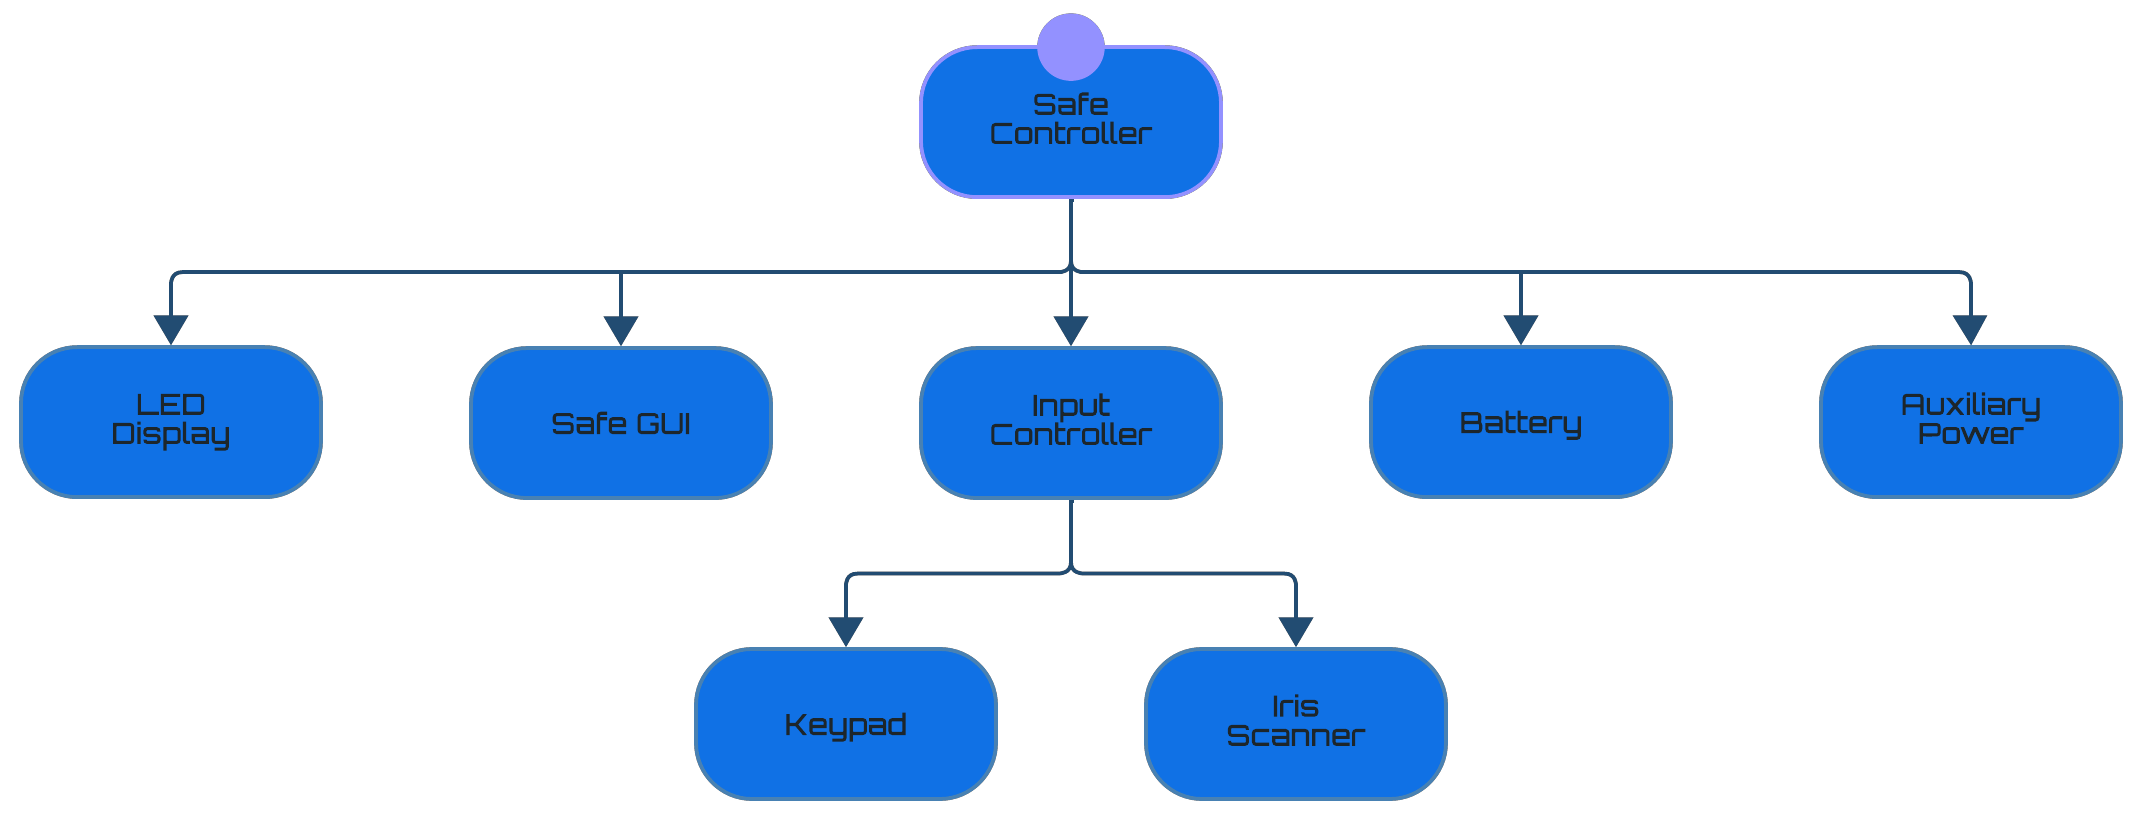
\includegraphics[scale=0.3]{docs/figs/architecture_design.png}
    \caption{Architecture Design Diagram \cite{lucidLucidVisual}}
    \label{fig:diagram1}
\end{figure}

\subsection{Design Description}
This section delves into the core software components: SafeController(), IrisScanner(), and Keypad() classes and their interactions. \\ \\
The SafeController() acts as the central command, promptly initializing the InputController(), Screen(), AuxPower(), and SafeGUI() components. When users present their eye to the biometric module, the IrisScanner() class springs into action, recognizing the eye pattern and sending the data to the InputController(). This data is then passed to the SafeController() for validation against stored iris patterns. \\ \\
Concurrently, the Keypad class oversees the user interactions with the keypad. When a user keys in a 6-digit PIN, the InputController() processes this input and coordinates with the SafeController() for verification, similar to the iris scanning procedure. \\ \\
After consolidating the authentication details, the SafeController() manages the overarching system dynamics. Depending on the verification outcomes, the SafeController() triggers reactions in the Screen(), Battery(), and tactile feedback mechanisms. These software components seamlessly bridge with their tangible equivalents: the display unit, power units, and the tactile feedback system of the keypad().

\section{Component Specifications}
This section delves into the intricacies of the software components illustrated in the design diagram outlined in Figure \ref{fig:diagram1}. It offers a comprehensive perspective on each software component and underscores their interdependencies.

\subsection{SafeController}
The \texttt{SafeController} class acts as the microcontroller in the software architecture. It manages the state of the safe and coordinates between different components, such as the LED Display, Keypad, and SafeGUI. It holds a list of users and maintains the current user and state.

\begin{itemize}
    \item \texttt{setState(SafeState newState)}: This method is used to change the state of the safe. It handles states like waiting for an iris scan, setting iris, initial PIN setup, normal, closed, adding a new user, locked, and master verification.
    \item \texttt{handleMasterVerification()}: This method is invoked when the state is set to master verification. It displays a message to enter the master PIN.
    \item \texttt{handleInitialPinSetup()}: and \texttt{handleNormalState()}: These methods handle the initial PIN setup and normal states by displaying appropriate messages.
    \item \texttt{handleUnlockedState()}: This method handles the unlocked state by displaying a message and opening the safe GUI after a delay.
    \item \texttt{checkPIN(String enteredPIN)}: This method checks the entered PIN against the stored PINs for various states and displays appropriate messages.
\end{itemize}
\textbf{Dependencies}:
\begin{itemize}
    \item Depends on the \texttt{Screen} class to display messages.
    \item Depends on the \texttt{SafeGUI} class to handle the GUI-related tasks.
    \item Depends on the \texttt{User} class to manage user information.
    \item Depends on the \texttt{SafeState} enum to manage the state of the safe.
\end{itemize}

\subsection{Input Controller}
The \texttt{InputController} class handles the input from the user via the IRIS scanner and Keypad. It manages the power state and interacts with the \texttt{Screen}, and \texttt{SafeController} to handle various inputs.

\begin{itemize}
    \item \texttt{handleKeyInput(String key)}: This method handles the key inputs from the user. If the power is on, it appends the key entry to the screen. Otherwise, it does nothing.
    \item \texttt{handleCancel()}: This method handles the cancel operation by removing the last key entry from the screen.
    \item \texttt{handleEnterButton()}: This method is invoked when the enter button is pressed. It checks the PIN entered by calling the \texttt{checkPIN} method of the \texttt{SafeController} and clears the key entry from the screen.
    \item \texttt{handlePowerButton()}: This method handles the power button press. It toggles the power state and sets the state of the \texttt{SafeController} accordingly.
\end{itemize}
\textbf{Dependencies}:
\begin{itemize}
    \item Depends on the \texttt{Screen} class to display and manage key entries.
    \item Depends on the \texttt{SafeController} class to check the PIN and set the state of the safe.
\end{itemize}

\subsection{GUI Manager (SafeGUI)}
The \texttt{SafeGUI} class is responsible for managing the graphical user interface of the safe. It handles the display of images representing the safe's state (open, closed), the keypad for PIN entry, and buttons for various controls.

\begin{itemize}
    \item \texttt{start(Stage primaryStage)}: This method initializes the primary stage of the application, setting up the images, button panel, screen, and keypad. It also handles mouse clicks on the image view to transition to a close-up view of the safe.
    \item \texttt{openSafe()}: This method changes the image to show the safe in an open state and hides the screen component, keypad, and button box. It also provides a button to close the safe.
    \item \texttt{closeSafe()}: This method is used to close the safe. It changes the state of the \texttt{safeController} to closed, updates the image to show the safe in a closed state, and makes the screen component, keypad, and button box visible again.
\end{itemize}
\textbf{Dependencies}:
\begin{itemize}
    \item Depends on the \texttt{Screen} class to manage the display screen of the safe.
    \item Depends on the \texttt{KeyPad} class for handling keypad-related operations.
    \item Depends on the \texttt{ButtonPanel} class for managing the button panel.
    \item Depends on the \texttt{SafeController} class to manage the state of the safe.
    \item Depends on the \texttt{SafeState} enum to manage the state of the safe.
\end{itemize}
This class is crucial for providing a user-friendly interface, allowing users to interact with the safe effectively and efficiently, and ensuring that the state of the safe is visually represented to the user at all times.

\subsection{Iris Scanner (Software)}
The Iris Scanner functionality is embedded within the \texttt{SafeController} class. It is responsible for handling the iris scanning and verification process to ensure secure access to the safe.

\begin{itemize}
    \item \texttt{handleWaitingForIris()}: This method displays a message on the screen indicating that the system is waiting for an iris scan.
    \item \texttt{handleSettingIris()}: This method prompts the user to scan their iris for setting or updating the iris data in the system.
    \item \texttt{checkIris(String irisName)}: This method checks the scanned iris data against the stored iris data for the current user. If the iris data matches, it transitions the state to unlocked; otherwise, it displays an error message and reverts to the normal state.
    \item \texttt{setIrisForCurrentUser(String irisName)}: This method sets the iris data for the current user in the system.
\end{itemize}
\textbf{Dependencies}:
\begin{itemize}
    \item Depends on the \texttt{Screen} class to display messages related to the iris scanning process.
    \item Depends on the \texttt{User} class to manage and verify user data, including iris data.
    \item Interacts with various states defined in the \texttt{SafeState} enum to manage the iris scanning and verification process flow.
\end{itemize}
This component ensures that only authorized users whose iris data matches the stored data can access the safe, providing an additional layer of security beyond the PIN authentication.

\subsection{Battery}

The \texttt{Battery} class in the software simulates the hardware component responsible for powering the safe and its associated features. It is essential for ensuring the continuous and reliable operation of the safe.

\begin{itemize}
    \item \texttt{start()}: This method begins the battery depletion process, continuously checking the battery level and updating the charge level.
    \item \texttt{stop()}: This method stops the battery depletion process and resets the timer.
    \item \texttt{discharge(double amount)}: This method discharges the battery by a specified amount.
    \item \texttt{isLow()}: This method checks if the battery is low based on the predefined low battery threshold.
    \item \texttt{getChargeLevel()}: This method returns the battery's current charge level.
\end{itemize}
\textbf{Dependencies}:

The \texttt{Battery} class does not depend on other classes but is crucial for the operation of any component that requires power to function. It uses the \texttt{Timer} and \texttt{TimerTask} classes to manage the battery depletion process.


\subsection{LED Display}
The \texttt{Screen} class represents the digital display of the safe. It provides functionalities to display messages, handle user input, and manage timeouts.

\begin{itemize}
    \item \texttt{displayMessage(String message)}: This method displays a given message on the screen. If the message is longer than 20 characters, it splits into two lines.
    \item \texttt{appendKeyEntry(String key)}: Appends a key entry (like a digit from a PIN) to the screen and represents it as an asterisk (*).
    \item \texttt{clearKeyEntry()}: Clears the current key entries displayed on the screen.
    \item \texttt{timeout()}: Handles the scenario when there's no activity on the screen for a certain duration. It clears the key entry and displays a "Timed out" message.
    \item \texttt{tempDisplayMessage(String message)}: Temporarily displays a message on the screen and then reverts to the previous message after a short duration.
    \item \texttt{removeLastKeyEntry()}: Removes the last key entry from the screen.
    \item \texttt{turnOn()}: Makes the screen visible.
    \item \texttt{turnOff()}: Makes the screen invisible.
    \item \texttt{getScreenComponent()}: Returns the main component of the screen, which is a \texttt{StackPane}.
\end{itemize}
\textbf{Dependencies}:
\begin{itemize}
    \item Depends on the \texttt{InputController} class to handle user input and manage the display accordingly.
    \item Uses \texttt{PauseTransition} from JavaFX to handle timeouts and temporary message displays.
\end{itemize}
The \texttt{Screen} class is essential for user interaction, providing feedback, and guiding the user through the various operations of the safe.



\section{Sample Use Cases}
This section offers two use cases showcasing varied scenarios involving HomeSafe. Each example elucidates the user's actions sequentially. Furthermore, with every user action, the reactions from the related system components are detailed.

\subsection{Use Case 1: Initial Setup}
\begin{itemize}
    \item \textbf{Actor}: User
    \item \textbf{Goal}: Successfully initialize and configure the HomeSafe with personalized access credentials.
    \item \textbf{Preconditions}: The HomeSafe is powered off and is in its initial, unconfigured state.
    \item \textbf{Trigger}: User powers on the HomeSafe.
    \item \textbf{Scenario}: In this scenario, the user has just acquired their new HomeSafe and wishes to initialize and configure their access credentials before turning off the safe for subsequent use.
    \begin{enumerate}
    \item \textbf{Unpacking and Placing the Safe}: User removes the HomeSafe and its manual, which contains the Master PIN, from the packaging, placing it in a preferred location.
    \item \textbf{Powering Up}: User powers up the system by pressing the power button, activating the safe's components and prompting an LED display message to enter the Master PIN.
    \item \textbf{Entering Master PIN}: User inputs the provided 6-digit Master PIN and presses ENTER, prompting the system to verify it and request the creation of a new personal PIN.
    \item \textbf{Setting a New Personal PIN}: User inputs a desired 6-digit PIN and presses ENTER.
    \item \textbf{Biometric (Iris) Configuration}: User aligns their eye with the Iris Scanner, waiting for the confirmation animation on the LED Display. This concludes the initial setup process, and the user's credentials are saved.
    \item \textbf{Powering Down}: The user presses the POWER button, deactivating the HomeSafe and all its internal components.
    \end{enumerate}
\end{itemize}

\subsection{Use Case 2: Accessing Contents of HomeSafe}
\begin{itemize}
    \item \textbf{Actor}: User
    \item \textbf{Goal}: Gain access to the HomeSafe utilizing pre-configured PIN and Iris Scan credentials.
    \item \textbf{Preconditions}:  The HomeSafe is configured with the user’s PIN and Iris Scan and is powered off.
    \item \textbf{Trigger}: The user wishes to access the contents of the HomeSafe.
    \item \textbf{Scenario}: The user, having previously configured their PIN and Iris Scan, seeks to gain secure access to the safe utilizing these credentials.
    \begin{enumerate}
    \item \textbf{Initiating Access}: The user begins by powering up the HomeSafe. The LED display comes to life, prompting the user to enter their 6-digit PIN to proceed.
    \item \textbf{PIN Verification}: The user enters their personal 6-digit PIN and presses ENTER. In response, the LED display instructs the user to perform an Iris Scan, activating the scanner.
    \item \textbf{Iris Scan Verification}: The user carefully positions their eye before the Iris Scanner. Upon seeing a confirmation animation on the LED Display which signifies a successful scan, the locking mechanism shifts to an UNLOCKED state.
    \item \textbf{Accessing and Managing Safe Contents}: With access granted, the user opens the safe, revealing its contents. The LED display notifies “Door Open”, deactivating input controls and initiating a timer that will sound an alarm if the door remains open beyond 300 seconds (5 minutes).
    \item \textbf{Securing the Safe Post-Use}: After managing the contents, the user closes the HomeSafe. The LED promptly indicates "Door Closed", reactivating the input controls and initializing a shutdown timer that will power down the safe after 300 seconds (5 minutes).
    \item \textbf{Concluding Interaction}: Optionally, to immediately cease all activity within the HomeSafe’s components, the user can manually power it down by pressing the POWER button.
    \end{enumerate}
\end{itemize}

\subsection{Use Case 3: PIN Timeout}
\begin{itemize}
    \item \textbf{Actor}: User
    \item \textbf{Goal}: To access the HomeSafe despite encountering a PIN entry timeout and subsequent system lockout.
    \item \textbf{Preconditions}: The HomeSafe is configured with the user’s PIN and Iris Scan and is powered off.
    \item \textbf{Trigger}: The user desires access to the HomeSafe but experiences interruption during PIN entry.
    \item \textbf{Scenario}: In an effort to access the HomeSafe, the user initiates the typical access protocol. However, they become subject to an unintended pause during PIN entry, initiating a timeout and subsequent challenges to regain access to the system.
    \begin{enumerate}
    \item \textbf{Initiating Access}: The user powers up the HomeSafe and begins entering their personal 6-digit PIN. The LED display lights up, showing each character of the partly entered PIN as asterisks (*) while an internal counter begins silently ticking down in the background.
    \item \textbf{Experiencing PIN Entry Timeout}: Due to a hesitation or interruption of over 3 seconds, the system enforces a timeout, resetting the PIN entry procedure and prompting the user once again for the 6-digit PIN via the LED display.
    \item \textbf{Encountering Consecutive Timeout Penalties}: After three consecutive timeout events, the HomeSafe takes a precautionary security measure, transitioning into a "LOCKED OUT" state. The LED display, adopting a more stringent security protocol, now requests the entry of the Master PIN.
    \item \textbf{Providing Master PIN to Resolve Lockout}:  In response to the "LOCKED OUT" state, the user enters the Master PIN as instructed. Successful verification removes the system from the lockout, reactivating standard access protocols.
    \item \textbf{Resuming Standard Access Procedure}: The LED display reverts to requesting the user’s personal 6-digit PIN, offering another opportunity to access the HomeSafe by proceeding with the authorization process.
    \end{enumerate}
\end{itemize}

\subsection{Use Case 4: Unauthorized Access (PIN)}
\begin{itemize}
    \item \textbf{Actor}: User
    \item \textbf{Goal}: To access the HomeSafe using established credentials while navigating through unauthorized access protocols upon multiple incorrect PIN entries.
    \item \textbf{Preconditions}:  The HomeSafe is configured with the user’s PIN and Iris Scan and is powered off.
    \item \textbf{Trigger}: The user intends to access the HomeSafe but fails to provide the correct PIN in multiple attempts.
    \item \textbf{Scenario}: The user, attempting to gain access to their HomeSafe, inadvertently fails to provide the correct PIN repeatedly. Subsequent incorrect entries enforce a system lockdown, prompting the user to establish their legitimacy by entering the Master PIN as a security override.
    \begin{enumerate}
    \item \textbf{Initiating Access}: The user powers up the HomeSafe, engaging the microcontroller and keypad. The LED display prompts the user for their 6-digit PIN.
    \item \textbf{Experiencing Failed PIN Entries}: The user enters an incorrect PIN and, upon pressing ENTER, is met with a failed verification message. This initiates an internal counter while the LED display prompts the user to try their 6-digit PIN again.
    \item \textbf{Encountering System Lockout due to Repeated Failures}: After three consecutive incorrect PIN entries, the HomeSafe, prioritizing security, transitions into a “LOCKED OUT” state. At this juncture, the LED display alters its request, now seeking the 6-digit Master PIN to proceed.
    \item \textbf{Overriding Lockout with Master PIN}: The user provides the Master PIN when requested. A successful entry recalibrates the system, lifting it from the “LOCKED OUT” state and reinstating the standard authorization protocols.
    \item \textbf{Resuming Standard Access Procedure}: With the lockout condition removed, the LED display reverts to requesting the user’s 6-digit PIN, allowing the user to proceed with the typical authorization process.
    \end{enumerate}
\end{itemize}

\subsection{Use Case 5: Unauthorized Access (Iris Scan)}
\begin{itemize}
    \item \textbf{Actor}: User
    \item \textbf{Goal}: Gain access to the HomeSafe despite encountering challenges with Iris Scan verification, utilizing the Master PIN as an override upon failed attempts.
    \item \textbf{Preconditions}:  The HomeSafe is configured with the user’s PIN and Iris Scan and is powered off.
    \item \textbf{Trigger}: The user seeks access to the HomeSafe but encounters difficulty with the Iris Scan verification process.
    \item \textbf{Scenario}: The user, having previously established both PIN and Iris Scan credentials, attempts to access the HomeSafe. A series of unsuccessful Iris Scan attempts propels the system into a secured "LOCKED OUT" state, prompting the user to affirm identity and intent via the Master PIN.
    \begin{enumerate}
    \item \textbf{Initiating Access}: The user powers up the HomeSafe, engaging the microcontroller and keypad. The LED display prompts the user for their 6-digit PIN.
    \item \textbf{PIN Verification}: he user enters their personal 6-digit PIN and presses ENTER. In response, the LED display instructs the user to perform an Iris Scan, activating the scanner.
    \item \textbf{Unsuccessful Iris Scan Attempts}: The user attempts the Iris Scan, but upon being determined as invalid, the LED display persists in its request for a valid Iris Scan.
    \item \textbf{Encountering System Lockout due to Repeated Failures}: After three continuous failed Iris Scan verifications, the HomeSafe enters a “LOCKED OUT” state. In this phase, the LED display modifies its prompt, now demanding the 6-digit Master PIN to override the lockout.
    \item \textbf{Overriding Lockout with Master PIN}: The user provides the Master PIN when requested. A successful entry recalibrates the system, lifting it from the “LOCKED OUT” state and reinstating the standard authorization protocols.
    \item \textbf{Resuming Standard Access Procedure}: With the lockout condition removed, the LED display reverts to requesting the user’s 6-digit PIN, allowing the user to proceed with the typical authorization process.
    \end{enumerate}
\end{itemize}

\newpage

\printbibliography

{\parindent0pt}

\end{document}
